\chapter{Implementation}

To make the cSVD algorithm easier to implement, a machine learning framework is used. Frameworks like TensorFlow (Google) \cite{tensorflow:about} and PyTorch (Facebook) \cite{pytorch:docs} were developed to simplify implementing machine learning applications. These machine learning frameworks make it easier to utilize the hardware on a single machine or a distributed network of machines \cite{pytorch:docs}. To implement the cSVD algorithm, PyTorch is used because it is easier to implement prototypes with it.  Depending on whether or not there is a GPU PyTorch uses different backends for computing. If there is no GPU available it uses MKL and LAPACK. If there is a GPU available it uses MAGMA with CUDA, thus only supporting NVIDIA GPUs \cite{pytorch:docs}. While using PyTorch without a GPU it is too slow for large computational problems and it is therefore beneficial to use the MAGMA version. PyTorch is also supported by the platform used for this project.

The platform used is the CLAAUDIA AI Cloud \footnote{\url{https://www.claaudia.aau.dk/platforms-tools/compute/gpu-cloud-ai/}}, which is a cluster consisting of three NVIDIA DGX-2. Each NVIDIA DGX-2 contains 16 NVIDIA V100 GPUs and 2x24 core Xeon CPUs. Figure \ref{fig:nvlink} shows the topology of each cluster. This is called NVLink and is a direct link between the GPUs so the communication does not have to go through the PCI bus, and for the V100 GPUs data is transferred 10 times faster than the PCI bus.

\begin{figure}[H]
  \centering
  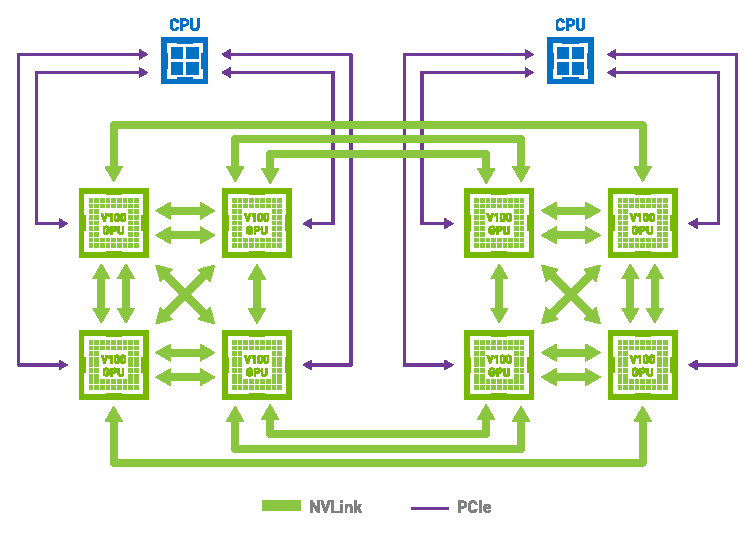
\includegraphics[scale=0.6]{Figures/nvlink.eps}
  \caption[]{NVLink\protect\footnotemark\ topology}
  \label{fig:nvlink}
\end{figure}
  
\footnotetext{\url{https://www.nvidia.com/en-us/data-center/nvlink/}}
  
The implementation strategy is to start out with a cSVD implementation that works sequentially, i.e. not supporting batch computation. This is then expanded upon until a fully batched version is implemented. The implementation will only use a single GPU on the cluster because of time constraints. The sequential implementation is based directly on the cSVD algorithm shown below, where $\Phi$ is now the shuffling random row sampling matrix, which is shown as simply selecting the first $l$ rows of the EDJM matrix $X$ in Algorithm \ref{alg:csvd:perm}.

$ $ \newline

\begin{algorithm}[H]
\SetAlgoLined
\SetKwInOut{Input}{Input}
\Input{Sparse matrix $X \in \mathbb{R}^{m \times N}$, target rank k and oversampling p}
$l \gets k + p$ \\
$Y \gets X[:l,:]$ \\
$B \gets Y Y^T$ \\
$B \gets \frac{1}{2}(B + B^T)$ \\
$T,D \gets \mathrm{eigs}(B,k)$ \\
$\tilde S \gets \sqrt{D}$ \\
$\tilde V \gets Y^T T \tilde S^{-1}$ \\
$\tilde U \gets X \tilde V$ \\
$U,S,Q^T \gets \mathrm{svd}(\tilde U)$ \\
$V \gets \tilde V Q$ \\
\KwResult{$U \in \mathbb{R}^{m \times k}$, $S \in \mathbb{R}^{k \times k}$, $V \in \mathbb{R}^{n \times k}$}
\caption{cSVD with $\Phi$ as a permutation matrix}
\label{alg:csvd:perm}
\end{algorithm}

$ $ \newline

The cSVD pseudocode depends on the function \texttt{eigs} which returns the first $k$ eigenvalues and eigenvectors in descending order. PyTorch \texttt{symeig} returns $l$ eigenvalues and eigenvectors in ascending order. To get the $k$ largest eigenvalues and eigenvectors in descending order, it is possible to select all the columns in opposite order. Algorithm \ref{alg:eigs} shows how \texttt{eigs} works.

$ $ \newline

\begin{algorithm}[H]
\SetAlgoLined
\SetKwInOut{Input}{Input}
\Input{$B \in \mathbb{R}^{l \times l}$, target rank k}
$T,D \gets \mathrm{symeig}(B)$ \#T is a matrix, D is a vector \\
$\mathrm{index} \gets [l-1, l-2,..., 0]$ \\
$D \gets \mathrm{select}(D, \mathrm{index})$ \#select columns indexed by index \\
$D \gets \mathrm{diag}(D[0:k])$ \#turn D into a diagonal matrix \\
$T \gets \mathrm{select}(T, \mathrm{index})$ \\
$T \gets T[:,0:k]$ \\
\KwResult{Eigenvectors $T \in \mathbb{R}^{k \times k}$, eigenvalues $D \in \mathbb{R}^{k \times k}$}
\caption{eigs}
\label{alg:eigs}
\end{algorithm}

$ $ \newline

The sequential implementation only works on single matrices rather than tensors. To implement a version that can compute the cSVD for batches of matrices, i.e. work on tensors, the implementation is modified to use PyTorch batch matrix multiplication. PyTorch does not support batch eigenvalue decomposition or batch SVD. The simple solution is to use for-loops on each matrix in the input tensor, as shown in Algorithm \ref{alg:forloop:batch:eigs} and \ref{alg:forloop:batch:svd}.

$ $ \newline

\begin{algorithm}[H]
\label{alg:forloop:batch:eigs}
\SetAlgoLined
\SetKwInOut{Input}{Input}
\Input{$B \in \mathbb{R}^{bs \times l \times l}$, target rank k}
$T \gets \mathrm{allocate}(\mathbb{R}^{bs \times k \times k})$ \\
$D \gets \mathrm{allocate}(\mathbb{R}^{bs \times k \times k})$ \\
\For{$i \gets 0$ \KwTo $bs$}{$T[i,:,:],D[i,:,:] \gets \mathrm{eigs}(B[i,:,:], k)$}
\KwResult{Eigenvectors $T \in \mathbb{R}^{bs \times k \times k}$, eigenvalues $D \in \mathbb{R}^{bs \times k \times k}$}
\caption{Batch-eigs (for-loop based)}
\end{algorithm}

$ $ \newline

\begin{algorithm}[H]
  \label{alg:forloop:batch:svd}
\SetAlgoLined
\SetKwInOut{Input}{Input}
\Input{$\tilde U \in \mathbb{R}^{bs \times m \times k}$, target rank k}
$U \gets \mathrm{allocate}(\mathbb{R}^{bs \times m \times k})$ \\
$S \gets \mathrm{allocate}(\mathbb{R}^{bs \times k \times k})$ \\
$Q \gets \mathrm{allocate}(\mathbb{R}^{bs \times k \times k})$ \\
\For{$i \gets 0$ \KwTo $bs$}{$U[i,:,:],S[i,:,:],Q[i,:,:] \gets \mathrm{svd}(\tilde U[i,:,:])$}
\KwResult{$U \in \mathbb{R}^{bs \times m \times k}$, $S \in \mathbb{R}^{bs \times k \times k}$, $Q \in \mathbb{R}^{k \times k}$}
\caption{Batch-SVD (for-loop based)}
\end{algorithm}

$ $ \newline

The next step in improving the cSVD is to use a real batch eigenvalue decomposition and SVD. PyTorch has a C++ API which makes it possible to use CUDA libraries, and then use \texttt{pybind11} to make Python bindings to that C++ code. This makes it possible to implement the majority of the algorithm using the PyTorch Python API and implement the required code for batching in C++ with Python bindings. PyTorch links against CUDA when using MAGMA, simplifying integration with \texttt{cuSOLVER}. It is possible to do batch eigenvalue decomposition with \texttt{cuSOLVER}, but not batch SVD with the exception of \texttt{gesvda} \cite{nvidia:cusolver} (only for tall matrices with a width of 100 or less).

CUDA and PyTorch use two different memory models, which is important to understand when mixing them. CUDA uses a column-major model and PyTorch uses a row-major model, shown in Figure \ref{fig:rowcol}. Whenever a matrix is passed between PyTorch and CUDA, it's necessary to transpose the matrix and make the data contiguous. When transposing matrices in PyTorch, no data is actually moved but this can be forced using the PyTorch API.

\begin{figure}[H]
    \centering
    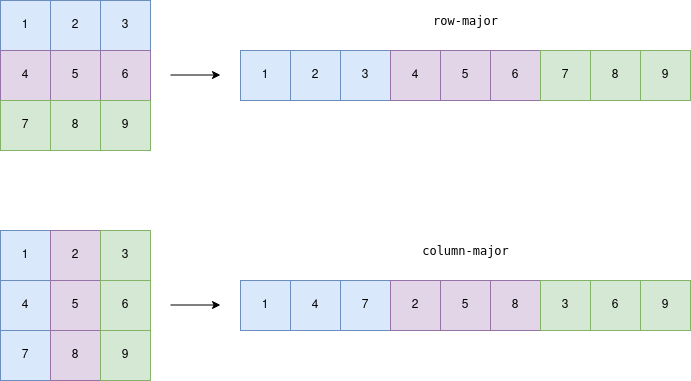
\includegraphics[scale=0.45]{Figures/major.png}
    \caption{Row- vs. column-major}
    \label{fig:rowcol}
\end{figure}

Two C++ function wrappers are implemented, the first is \texttt{batch\_symeig} which uses \texttt{cuSOLVER}'s batched symmetric eigenvalue decomposition to compute the eigenvalues in batch, the second is a wrapper around cuSOLVER's \texttt{gesvda}. Using pybind11, Python bindings are generated for these two wrapper functions, which can then be used from PyTorch.

To integrate the cSVD algorithm better with PyTorch, it can be wrapped in a PyTorch \texttt{Function} class. PyTorch functions are represented as classes with a \texttt{forward} (forward propagation) and \texttt{backward} (backward propagation) method as Figure \ref{fig:pytorch:function} shows. A useful feature of PyTorch is the Automatic Differentiation (Autograd) \cite{pytorch:docs}, as it can automatically calculate the gradient for any combination of differentiable functions. The \texttt{backward} method is automatically derived when using the Python API, but not when using the C++ API. So when using the C++ API it has to be manually implemented.

\begin{figure}[H]
    \centering
    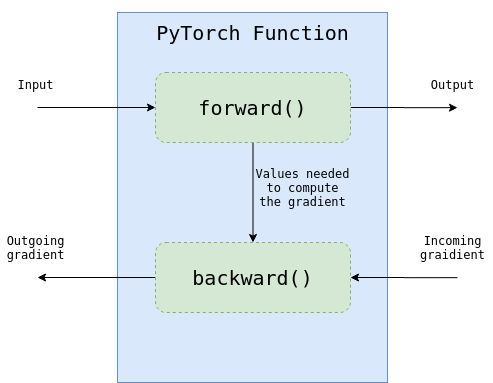
\includegraphics[scale=0.45]{Figures/pytorch_function.png}
    \caption{PyTorch Function class overview}
    \label{fig:pytorch:function}
\end{figure}

Autograd works by building a tree of functions, when \texttt{forward} is called, the tree is expanded. Forward for an SVD would create three branches, one for each matrix output. When \texttt{backward} is called, the tree can be traversed backwards, each leaf in the tree has its gradient calculated which is then fed backward. Thus the \texttt{backward} method for an SVD would receive three matrices as an input, and based on that calculate a gradient for the original SVD input. By implementing support for batching of matrices, it can compute the cSVD for many matrices in parallel. Ideally this would be done purely in Python as it can automatically derive the \texttt{backward} method and it speeds up development. But there is a method to make the \texttt{backward} for the cSVD implementation faster. To increase performance one \texttt{backward} in C++ for the whole cSVD is implemented, rather than making individual \texttt{backward} implementations to the C++ symmetric eigenvalue decomposition and \texttt{gesvda}.